\documentclass[11pt]{article}%设置文档类型{article}和字体大小{11pt}，适配本地字体

\usepackage[a4paper]{geometry}%页面布局，纸张大小[a4paper]
\geometry{left=2.0cm,right=2.0cm,top=2.5cm,bottom=2.5cm}%页面边距
\usepackage[UTF8]{ctex}%latex支持中文宏包
\usepackage{amsmath, amsfonts, amssymb, amsthm}%数学公式环境、数学字体、数学字体扩展包、定理环境
\usepackage{bm,mathtools}%数学粗体、amsmath扩展包
\usepackage{graphicx}%插入和管理图片
\usepackage[graphicx]{realboxes}%创建和管理盒子（装有文本和图形）
\usepackage{algorithm,algorithmicx}%支持伪代码宏包
\usepackage[noend]{algpseudocode}%支持伪代码宏包
\usepackage{fancyhdr}%定制页眉和页脚
\setlength{\headheight}{13.6pt}%避免页眉高度警告
\pagestyle{fancy}
\fancyhf{} % 清空默认的页眉和页脚
\fancyhead[L]{\kaishu 中国科学院大学}
\fancyhead[C]{林俊杰2023K8009916012}
\fancyhead[R]{\kaishu}
\fancyfoot[C]{\thepage}
\usepackage{booktabs}%美化表格宏包
\usepackage{caption}%定制图表标题宏包
\usepackage{xcolor}%切换字体颜色
\usepackage{placeins}%控制浮动体位置
\usepackage{cleveref}%智能引用
\crefname{figure}{图}{figures}
\Crefname{figure}{Figure}{Figures}
\crefname{table}{表}{tables}
\Crefname{table}{Table}{Tables}
\usepackage{tikz} % 绘图宏包
\usetikzlibrary{arrows.meta, positioning, calc, shapes, fit, decorations.pathreplacing} % 加载绘图库
\usepackage{tikz-3dplot} %%三维图形绘制需要的宏包
\usetikzlibrary{patterns}%%填充使用的宏包 

%数学环境计数器
\newcounter{counter_exm}\setcounter{counter_exm}{1}
%\newcounter{counter_thm}\setcounter{counter_thm}{1}
%\newcounter{counter_lma}\setcounter{counter_lma}{1}
%\newcounter{counter_dft}\setcounter{counter_dft}{1}
%\newcounter{counter_clm}\setcounter{counter_clm}{1}
%\newcounter{counter_cly}\setcounter{counter_cly}{1}

%图标随章节计数{章节.张数}
\counterwithin{figure}{section}
\counterwithin{table}{section}

\newtheorem{theorem}{{\hskip 1.7em \bf 定理}}
\newtheorem{lemma}[theorem]{\hskip 1.7em 引理}
\newtheorem{proposition}[theorem]{Proposition}
\newtheorem{claim}[theorem]{\hskip 1.7em 命题}
\newtheorem{corollary}[theorem]{\hskip 1.7em 推论}
\newtheorem{definition}[theorem]{\hskip 1.7em 定义}

\renewcommand{\emph}[1]{{\kaishu #1}}
\newcommand{\articlename}{Stirling 公式}

\newenvironment{solution}{{\noindent\hskip 2em \bf 解 \quad}}{\par}
\newenvironment{example}{{\noindent\hskip 2em \bf 例 \arabic{counter_exm}\quad}}{\addtocounter{counter_exm}{1}\par}
\newenvironment{concept}[1]{{\bf #1\quad} \begin{kaishu}}{\end{kaishu}\par}
\renewenvironment{proof}{{\noindent\hskip 2em \bf 证明 \quad}}{\hfill$\qed$\par}

\begin{document}
    \begin{center}
        \LARGE \bf \articlename
    \end{center}

    \section{Stirling公式}

    Stirling公式描述了阶乘在 \(n\to\infty\) 时的渐近行为。

    最常见的形式是

    \[
    \boxed{
    n!
    \sim
    \sqrt{2\pi n}
    \left(\frac{n}{e}\right)^n
    }
    \]

    \vspace{1em}
    两边取对数可得

    \[
    \boxed{
    \log n!
    =
    \left(n+\frac12\right)\log n
    -n
    +\frac12\log(2\pi)
    +o(1)
    }
    \]

    \vspace{1em}
    更进一步，可以得到完整的渐近展开

    \[
    \boxed{
    \log n!
    \sim
    \left(n+\frac12\right)\log n
    -n
    +\frac12\log(2\pi)
    +\frac1{12n}
    -\frac1{360n^3}
    +\frac1{1260n^5}
    -\frac1{1680n^7}
    +\cdots
    }
    \]

    \vspace{1em}
    上述级数中的系数可以写成统一形式

    \[
    \boxed{
    \log n!
    \sim
    \left(n+\frac12\right)\log n
    -n
    +\frac12\log(2\pi)
    +
    \sum_{k=1}^{\infty}
    \frac{B_{2k}}
        {2k(2k-1)n^{2k-1}}
    }
    \]

    \vspace{1em}
    其中 \(B_{2k}\) 为 Bernoulli 数。

    本笔记的目标是从最粗糙的近似

    \[
    \log n!
    \approx
    n\log n-n
    \]

    \vspace{1em}
    出发，逐步推导出

    \[
    \frac12\log n
    \qquad
    \frac1{12n}
    \qquad
    -\frac1{360n^3}
    \qquad
    \ldots
    \]

    \vspace{1em}
    等修正项，最终得到 Stirling 公式的完整渐近展开。

    \section{积分估计得到主项}

    \begin{figure}[H]
        \centering
        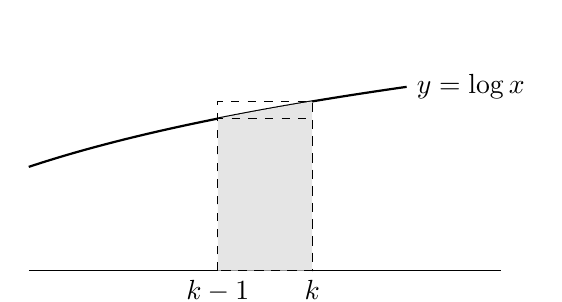
\begin{tikzpicture}[scale=1.2]

            % 坐标轴
            \draw (3,0) -- (8,0) ;

            % log 曲线
            \draw[thick,domain=3:7,smooth,samples=200]
            plot (\x,{ln(\x)})
            node[right] {$y=\log x$};

            % 区间
            \def\a{5}
            \def\b{6}

            % 曲线下真实面积
            \fill[gray!20]
            (\a,0)
            --
            plot[domain=\a:\b,samples=100]
            (\x,{ln(\x)})
            --
            (\b,0)
            -- cycle;

            % 左矩形
            \draw[dashed]
            (\a,0)
            rectangle
            (\b,{ln(\a)});

            % 右矩形
            \draw[dashed]
            (\a,0)
            rectangle
            (\b,{ln(\b)});

            % 端点
            \draw (\a,0) node[below] {$k-1$};
            \draw (\b,0) node[below] {$k$};

        \end{tikzpicture}
        \caption{积分估计}
        \label{fig:stirling_integral_estimate}
    \end{figure}

    \[
    \log n!
    =
    \sum_{k=1}^{n}\log k
    \]

    \vspace{1em}
    由于函数

    \[
    f(x)=\log x
    \]

    \vspace{1em}
    在 \((0,+\infty)\) 上单调递增，因此对于每个区间
    \([k-1,k]\) 有
    
    \[
    \log(k-1)
    \leqslant
    \int_{k-1}^{k}\log x\,dx
    \leqslant
    \log k
    \]

    \vspace{1em}
    对 \(k=2,\ldots,n\) 求和

    \[
    \sum_{k=2}^{n}\log(k-1)
    \leqslant
    \sum_{k=2}^{n}
    \int_{k-1}^{k}\log x\,dx
    \leqslant
    \sum_{k=2}^{n}\log k
    \]

    \vspace{1em}
    即

    \[
    \log (n-1)!
    =
    \sum_{k=1}^{n-1}\log k
    \leqslant
    \int_{1}^{n}\log x\,dx
    \leqslant
    \sum_{k=2}^{n}\log k
    =
    \log n!
    \]

    \vspace{1em}
    得到

    \[
    \boxed{
    \log (n-1)!
    \leqslant
    \int_{1}^{n}\log x\,dx
    \leqslant
    \log n!
    }
    \]

    \vspace{1em}
    下面计算积分

    \[
    \begin{aligned}
    \int_{1}^{n}\log x\,dx
    &=
    \Bigl[x\log x-x\Bigr]_{1}^{n}
    \\
    &=
    n\log n-n+1
    \end{aligned}
    \]

    \vspace{1em}
    代入前面的不等式

    \[
    \log (n-1)!
    \leqslant
    n\log n-n+1
    \leqslant
    \log n!
    \]

    \vspace{1em}
    又因为

    \[
    \log n!
    =
    \log (n-1)!+\log n
    \]

    \vspace{1em}
    所以

    \[
    \boxed{
    n\log n-n+1
    \leqslant
    \log n!
    \leqslant
    n\log n-n+1+\log n
    }
    \]

    \vspace{1em}
    于是

    \[
    0
    \leqslant
    \log n!
    -
    (n\log n-n)
    \leqslant
    \log n+1
    \]

    因此

    \[
    \boxed{
    \log n!
    =
    n\log n-n+O(\log n)
    }
    \]

    这说明
    \(\log n!\) 的主项为

    \[
    \boxed{
    n\log n-n
    }
    \]

    后续需要进一步研究误差项

    \[
    G(n)
    =
    \log n!
    -(n\log n-n)
    \]

    才能得到 Stirling 公式中的

    \[
    \frac12\log n
    \qquad
    \frac1{12n}
    \qquad
    -\frac1{360n^3}
    \qquad
    \ldots
    \]

    等更精细的修正项。

    \section{利用递推关系推导 Stirling 展开}

    我们从最粗糙的近似开始：

    \[
    \log n!
    \approx
    n\log n-n
    \]

    \vspace{1em}
    定义误差项

    \[
    G(n)
    =
    \log n!
    -
    (n\log n-n)
    \]

    \vspace{1em}
    我们的目标是研究 \(G(n)\) 的渐近行为。

    \subsection{误差的递推关系}

    \[
    \begin{aligned}
    G(n+1)-G(n)
    =
    \log(n+1)
    -
    \Bigl[(n+1)\log(n+1)-(n+1)\Bigr]
    +
    \Bigl[n\log n-n\Bigr]
    \end{aligned}
    \]

    \vspace{1em}
    整理得

    \[
    \boxed{
    G(n+1)-G(n)
    =
    1-n\log\!\left(1+\frac1n\right)
    }
    \]

    \subsection{差分展开}

    利用

    \[
    \log(1+x)
    =
    x-\frac{x^2}{2}
    +\frac{x^3}{3}
    -\frac{x^4}{4}
    +\cdots
    \]

    \vspace{1em}
    代入 \(x=\frac1n\)，得到

    \[
    \log\!\left(1+\frac1n\right)
    =
    \frac1n
    -\frac1{2n^2}
    +\frac1{3n^3}
    -\frac1{4n^4}
    +\cdots
    \]

    \vspace{1em}
    乘以 \(n\)

    \[
    n\log\!\left(1+\frac1n\right)
    =
    1-\frac1{2n}
    +\frac1{3n^2}
    -\frac1{4n^3}
    +\cdots
    \]

    \vspace{1em}
    因此

    \[
    \boxed{
    G(n+1)-G(n)
    =
    \frac1{2n}
    -\frac1{3n^2}
    +\frac1{4n^3}
    -\frac1{5n^4}
    +\cdots
    }
    \]

    \subsection{发现 $\frac12\log n$}

    注意

    \[
    \log(n+1)-\log n
    =
    \log\!\left(1+\frac1n\right)
    =
    \frac1n+O\!\left(\frac1{n^2}\right)
    \]

    \vspace{1em}
    因此

    \[
    \varDelta(\log n)
    \sim
    \frac1n
    \]

    \vspace{1em}
    而

    \[
    G(n+1)-G(n)
    \sim
    \frac1{2n}
    \]

    \vspace{1em}
    于是自然猜测

    \[
    G(n)
    \sim
    \frac12\log n
    \]

    \vspace{1em}
    定义

    \[
    F(n)
    =
    G(n)-\frac12\log n
    \]

    \vspace{1em}
    即

    \[
    \boxed{
    F(n)
    =
    \log n!
    -
    \left(n+\frac12\right)\log n
    +n
    }
    \]

    \subsection{新的差分方程}

    \[
    F(n+1)-F(n)
    =
    \bigl[G(n+1)-G(n)\bigr]
    -\frac12
    \log\!\left(1+\frac1n\right)
    \]

    \vspace{1em}
    代入前面的展开

    \[
    \begin{aligned}
    F(n+1)-F(n)
    =
    &\left(
    \frac1{2n}
    -\frac1{3n^2}
    +\frac1{4n^3}
    -\frac1{5n^4}
    +\cdots
    \right)
    \\
    -
    &\left(
    \frac1{2n}
    -\frac1{4n^2}
    +\frac1{6n^3}
    -\frac1{8n^4}
    +\cdots
    \right)
    \end{aligned}
    \]

    \vspace{1em}
    整理得到

    \[
    \boxed{
    F(n+1)-F(n)
    =
    -\frac1{12n^2}
    +\frac1{12n^3}
    -\frac3{40n^4}
    +\frac1{15n^5}
    +\cdots 
    }
    \]

    \vspace{1em}
    由于右边已经没有 \(1/n\) 项，因此 \(F(n)\) 趋向常数。

    \subsection{假设负幂展开}

    设

    \[
    \boxed{
    F(n)
    =
    C
    +\frac{a_1}{n}
    +\frac{a_2}{n^2}
    +\frac{a_3}{n^3}
    +\cdots
    }
    \]

    \vspace{1em}
    下面利用差分方程求出这些系数。

    \subsection{展开 $(n+1)^{-k}$}

    \[
    \begin{aligned}
    (n+1)^{-k}
    &=
    \left[n\left(1+\frac{1}{n}\right)\right]^{-k} \\
    &=
    n^{-k}\left(1+\frac{1}{n}\right)^{-k}
    \end{aligned}
    \]

    \vspace{1em}
    由广义二项式展开

    \[
    (1+x)^\alpha
    =
    1+\alpha x
    +\frac{\alpha(\alpha-1)}{2!}x^2
    +\frac{\alpha(\alpha-1)(\alpha-2)}{3!}x^3
    +\cdots
    \]

    \vspace{1em}
    令

    \[
    \alpha=-k \qquad x=\frac{1}{n}
    \]

    \vspace{1em}
    得到

    \[
    \begin{aligned}
    \left(1+\frac{1}{n}\right)^{-k}
    &=
    1-\frac{k}{n}
    +\frac{k(k+1)}{2n^2}
    -\frac{k(k+1)(k+2)}{6n^3}
    +\cdots
    \end{aligned}
    \]

    \vspace{1em}
    因此

    \[
    \boxed{
    \frac{1}{(n+1)^k}
    -
    \frac{1}{n^k}
    =
    -\frac{k}{n^{k+1}}
    +\frac{k(k+1)}{2n^{k+2}}
    -\frac{k(k+1)(k+2)}{6n^{k+3}}
    +\cdots
    }
    \]

    \vspace{1em}
    代入 \(k=1\)

    \[
    \boxed{
    \frac{1}{n+1}
    -
    \frac{1}{n}
    =
    -\frac{1}{n^2}
    +\frac{1}{n^3}
    -\frac{1}{n^4}
    +\cdots
    }
    \]

    \vspace{1em}
    同理

    \[
    \boxed{
    \frac1{(n+1)^2}-\frac1{n^2}
    =
    -\frac2{n^3}
    +\frac3{n^4}
    -\frac4{n^5}
    +\cdots
    }
    \]

    \vspace{1em}
    以及

    \[
    \boxed{
    \frac1{(n+1)^3}-\frac1{n^3}
    =
    -\frac3{n^4}
    +\frac6{n^5}
    -\frac{10}{n^6}
    +\cdots
    }
    \]

    \subsection{比较系数}

    \[
    \begin{aligned}
    F(n+1)-F(n)
    &=
    a_1
    \left(
    -\frac1{n^2}
    +\frac1{n^3}
    -\frac1{n^4}
    +\cdots
    \right)
    +
    a_2
    \left(
    -\frac2{n^3}
    +\frac3{n^4}
    +\cdots
    \right)
    +
    a_3
    \left(
    -\frac3{n^4}
    +\cdots
    \right)
    +\cdots \\
    &=
    -\frac{a_1}{n^2}
    +\frac{a_1-2a_2}{n^3}
    -\frac{a_1-3a_2+3a_3}{n^4}
    +\cdots
    \end{aligned}
    \]

    \vspace{1em}
    与

    \[
    -\frac1{12n^2}
    +\frac1{12n^3}
    -\frac3{40n^4}
    +\cdots
    \]

    \vspace{1em}
    逐项比较。

    比较 \(n^{-2}\)

    \[
    -a_1
    =
    -\frac1{12}
    \]

    \vspace{1em}
    因此

    \[
    \boxed{
    a_1=\frac1{12}
    }
    \]

    \vspace{1em}
    比较 \(n^{-3}\)

    \[
    a_1-2a_2
    =
    \frac1{12}
    \]

    \vspace{1em}
    代入 \(a_1\)，得到

    \[
    \boxed{
    a_2=0
    }
    \]

    \vspace{1em}
    比较 \(n^{-4}\)

    \[
    -a_1+3a_2-3a_3
    =
    -\frac3{40}
    \]

    \vspace{1em}
    代入前面结果

    \[
    -\frac1{12}-3a_3
    =
    -\frac3{40}
    \]

    \vspace{1em}
    解得

    \[
    \boxed{
    a_3=-\frac1{360}
    }
    \]

    \subsection{得到前几项 Stirling 展开}

    因此

    \[
    F(n)
    =
    C
    +\frac1{12n}
    -\frac1{360n^3}
    +\cdots
    \]

    \vspace{1em}
    代回

    \[
    F(n)
    =
    \log n!
    -
    \left(n+\frac12\right)\log n
    +n
    \]

    \vspace{1em}
    得到

    \[
    \boxed{
    \log n!
    =
    \left(n+\frac12\right)\log n
    -n
    +C
    +\frac1{12n}
    -\frac1{360n^3}
    +\cdots
    }
    \]

    \vspace{1em}
    其中常数

    \[
    C
    =
    \frac12\log(2\pi)
    \]

    \vspace{1em}
    可通过 Wallis 公式、Gamma 函数或中心二项式系数进一步确定。

    最终得到 Stirling 渐近展开

    \[
    \boxed{
    \log n!
    \sim
    \left(n+\frac12\right)\log n
    -n
    +\frac12\log(2\pi)
    +\frac1{12n}
    -\frac1{360n^3}
    +\cdots
    }
    \]
\end{document}